%---------------------------------------------------
% Nombre: capitulo2.tex  
% 
% Texto del cap�tulo 2
%---------------------------------------------------

\chapter{Experimento de datos}
\label{dos}

En este cap�tulo, realizaremos las consultas sobre la base de datos para ello, nos pondremos en lugar de un hipot�tico cient�fico de datos para obtener informaci�n acerca de las quejas de los usuarios.

\section{Creaci�n de la base de datos}

Para poder generar las consultas sin interferir con las dem�s que se realicen en el cluster crearemos una base de datos propia. 

Para ello, una vez dentro del cluster de Hadoop, primero conectamos a impala-shell. Tras esto, podemos crear la base de datos:

{\small
\begin{verbatim}
CREATE DATABASE CD_DNI IF NOT EXISTS
LOCATION '/user/impala/CD_DNI/impalastore.db';
\end{verbatim}
}
	
Una vez creada, podemos mostrarla y usarla:

{\small
\begin{verbatim}
DESCRIBE CD_DNI
USE CD_DNI
\end{verbatim}
}

\section{Carga de los datos}

Una vez creada la base de datos debemos cargar los datos en la misma, para ello, primero deberemos mandar los datos al HDFS de hadoop.

{\small
\begin{verbatim}
hdfs dfs -put ConsumerComplaints.csv /user/impala/CD_DNI/input
hdfs dfs -ls /user/impala/CD_DNI/input
\end{verbatim}
}

Si todo a ido bien, observaremos que la base de datos ahora est� en el hdfs de hadoop, por lo que podremos cargar los datos en una tabla, para ello cargamos el impala-shell y usamos (comando USE) nuestra base de datos creada anteriormente. 

{\small
\begin{verbatim}
CREATE TABLE IF NOT EXISTS Complaints(DateReceived STRING, 
ProductName STRING, SubProduct STRING,Issue STRING, SubIssue
STRING,ConsumerComplaintNarrative STRING,CompanyPublicResponse 
String, Company STRING, StateName STRING,ZipCode INT, Tags STRING,
ConsumerConsentProvided STRING,SubmittedVia STRING, DateSenttoCompany
STRING, CompanyResponsetoConsumer STRING, TimelyResponse STRING,
ConsumerDisputed STRING, ComplaintID INT) ROW FORMAT DELIMITED FIELDS
TERMINATED BY '\,' STORED AS TEXTFILE;
\end{verbatim}
}

Tras esto  \textbf{cargamos los datos}.

{\small
\begin{verbatim}
LOAD DATA INPATH '/user/impala/CD_DNI/input/ConsumerComplaints.csv' 
OVERWRITE INTO TABLE complaints;
\end{verbatim}
}

Tras esto en la figura \ref{1} podemos ver que la carga de datos se ha llevado a cabo correctamente. 


\begin{figure}[H]
	\centering
		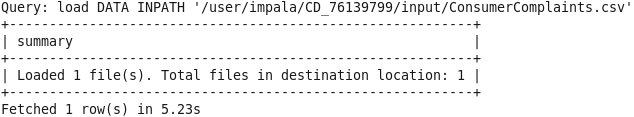
\includegraphics[scale=0.5]{./Capitulo2/imagenes/1.png}
		\caption{Carga de datos.}
	\label{1}
\end{figure}

\section{Proceso exploratorio}

Somos nuevos en la compa��a y queremos saber:

\textit{\textbf{�Cuales son las posibles fuentes de queja de nuestros usuarios?}}

{\small
\begin{verbatim}
SELECT DIFFERENT SubmittedVia FROM complaints;
\end{verbatim}
}

Parece que la salida ofrece m�s resultados de los que cabr�a esperar, por lo que de momento, hemos descubierto que la tabla en origen tiene datos de otras columnas introducidos err�neamente. Esto es algo que deber�amos solventar y arreglar en los datos a�n as�, buscaremos aquellas v�as que son m�s comunes haciendo uso de conteos para evitarnos cierto ruido y dar respuesta a la hipot�tica pregunta a resolver. 

{\small
\begin{verbatim}
SELECT COUNT(*), SubmittedVia FROM complaints 
	GROUP BY SubmittedVia HAVING COUNT(*) > 300;
\end{verbatim}
}

La salida de la consulta  podemos verla en la figura \ref{2}. 

\begin{figure}[H]
	\centering
		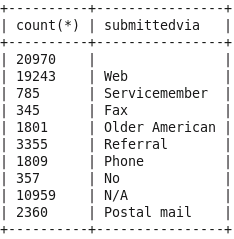
\includegraphics[scale=0.5]{./Capitulo2/imagenes/2.png}
		\caption{Salida de la consulta 1.}
	\label{2}
\end{figure}

Parece que as� ya sabemos cuales son las m�s comunes, igualmente siguen apareciendo algunas que no nos interesan por lo que utilizaremos WHERE para eliminarlas y ordenaremos para crear un ranking de las m�s usadas. 

{\small
\begin{verbatim}
SELECT COUNT(*), SubmittedVia FROM complaints GROUP BY
SubmittedVia WHERE SubmittedVia IN ('Web', 'Phone', 'Fax', 'Postal mail')
HAVING COUNT(*) > 300 ORDER BY 1 DESC;
\end{verbatim}
}

La salida de la consulta  podemos verla en la figura \ref{3}. 

\begin{figure}[H]
	\centering
		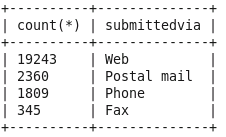
\includegraphics[scale=0.6]{./Capitulo2/imagenes/3.png}
		\caption{Salida de la consulta 2.}
	\label{3}
\end{figure}


Ya sabemos cuales son aquellos m�todos m�s usados para comunicarse con la empresa, pero ahora se nos encarga obtener aquellos estados en los cuales la gente usa menos la web para comunicarse con la empresa con el fin de potenciar la publicidad de una nueva aplicaci�n web de la compa��a. 

{\small
\begin{verbatim}
SELECT COUNT(*), SatateName FROM complaints GROUP BY
SubmittedVia WHERE SubmittedVia = 'Web' HAVING COUNT(*) < 10;
\end{verbatim}
}

La salida de la consulta  podemos verla en la figura \ref{4}. 

\begin{figure}[H]
	\centering
		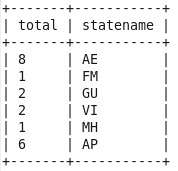
\includegraphics[scale=0.6]{./Capitulo2/imagenes/4.png}
		\caption{Salida de la consulta 3.}
	\label{4}
\end{figure}


Sabemos por tanto que los estados que menos usan la web son: AE (Fuerzas armadas en Africa), 	FM (Los estados de la micronesia), GU (Guam), MH (Las Islas Marshall) y VI  (Islas Virgenes) y AP (Las fuerzas armadas del pac�fico).

Esto nos ayuda poco, pues podemos comprobar que son casos aislados de soldados o personas destinadas en islas, y nosotros estamos interesados en los estados m�s relevantes de estados Unidos donde ofrecer nuestro nuevo producto por ello, exigiremos un m�nimo de comunicaciones para evitar estos casos aislados, o outliers en nuestro problema.


{\small
\begin{verbatim}
SELECT COUNT(*), SatateName FROM complaints GROUP BY
SubmittedVia WHERE SubmittedVia = 'Web' HAVING COUNT(*) BETWEEN 100 and 200;
\end{verbatim}
}


La salida de la consulta  podemos verla en la figura \ref{5}. 

\begin{figure}[H]
	\centering
		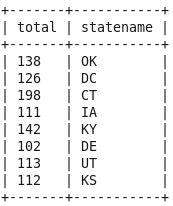
\includegraphics[scale=0.6]{./Capitulo2/imagenes/5.png}
		\caption{Salida de la consulta 4.}
	\label{5}
\end{figure}

El resultado de esta consulta nos dice cuales son aquellos estados que menos usan la web, por lo que aqu� deber�amos potenciar nuestro producto, si los analizamos, excepto Delawere, los dem�s son estados de predominio rural algo que era de esperar.

\pagebreak
\clearpage
%---------------------------------------------------